\chapter{ROS tools en etc.}
In de afbeeldingen \ref{fig:topics} en \ref{fig:service} zien we meerdere nodes en verbindingen die aangeven hoe de nodes met elkaar communiceren. Dergelijke figuren noemen we een \textit{communication graph} van de architectuur van het systeem. Deze type afbeeldingen geven de stroom van informatie aan en welke nodes afhankelijk zijn van welke nodes. Als we naar een groter systeem gaan, zoals te zien in figuur \ref{fig:architectuur-WOR1920-S2}, wordt het lastiger om hier goed overzicht van te houden. Er zijn verschillende manieren om toch overzicht te houden, waaronder de belangrijkste: het modelleren van het systeem. Gelukkig biedt ook ROS 2 hier ons hulpmiddelen bij. Bekijk daarom goed wat er allemaal mogelijk is met ROS via de commandline. Naast de hulpmidellen voor modelleren biedt de ROS 2 commandline commando's ook opties voor testen, analyseren en beheer. In de volgende sectie geven we een zeer incomplete lijst van de mogelijkheden.

\begin{figure}[ht]
\begin{center}
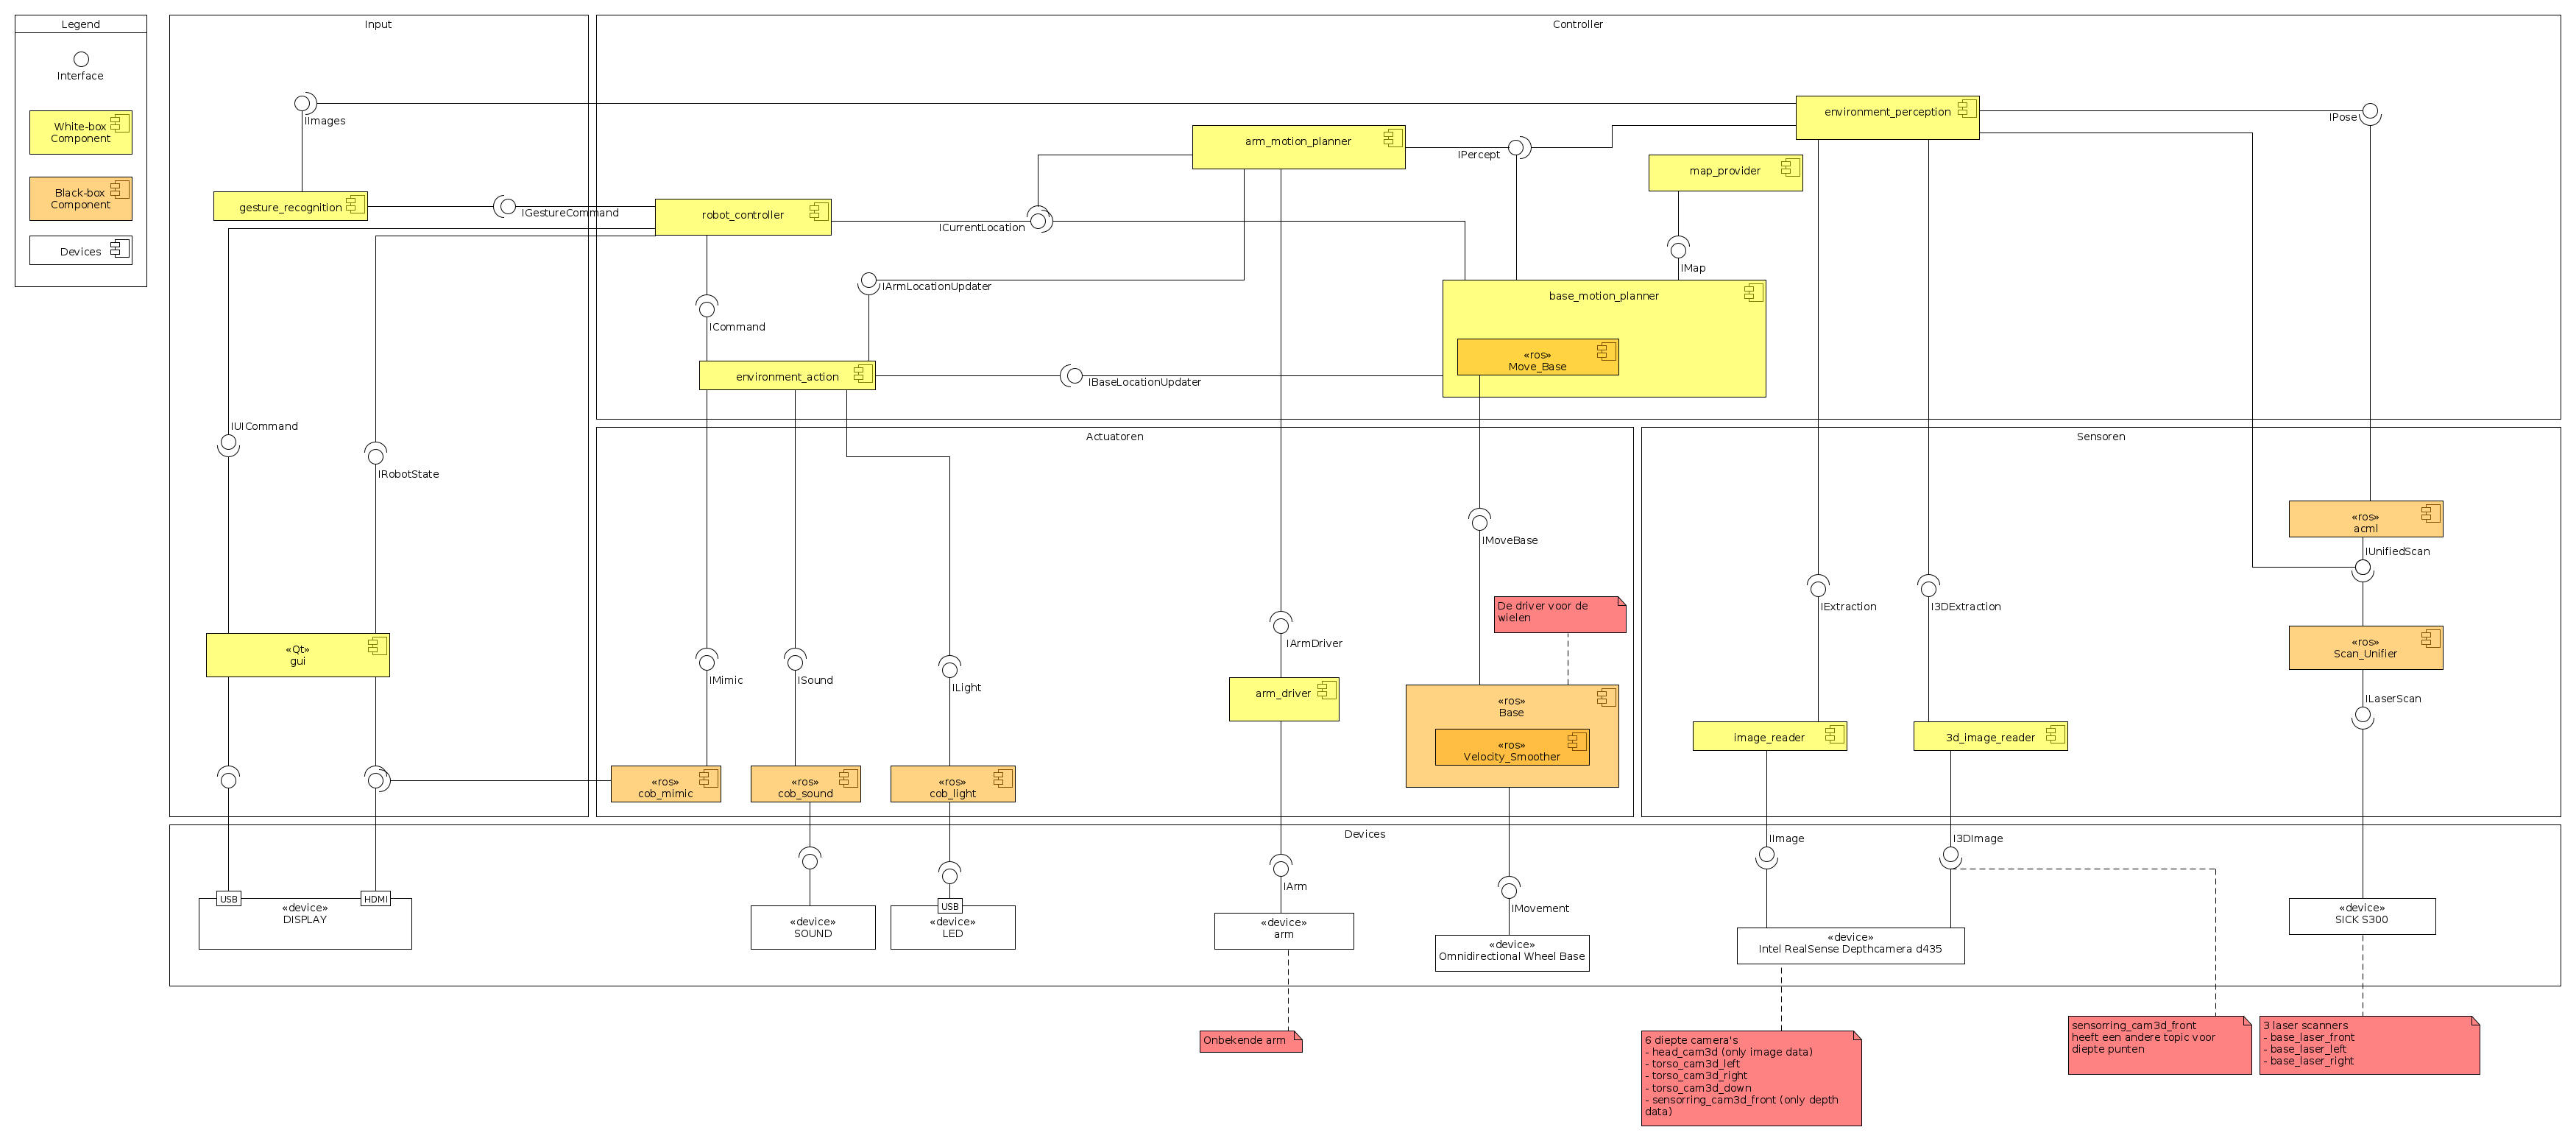
\includegraphics[scale=0.18, angle=-90, origin=c]{architectuur-WOR1920-S2}\\
\end{center}
\caption{De architectuur van het \textit{World Of Robots}-project van 19-20 S2 bij de opleiding ESD aan de HAN.}\label{fig:architectuur-WOR1920-S2}
\end{figure}

\section{Handige ROS commando's}
ROS komt allerlei handige commando's om je packages te bouwen en te onderhouden. In table \ref{table:ROS_commandos} staan er een aantal. Weet jij een commando die hier aan moet worden toegevoegd, neem dan vooral contact op met de auteur. 

\begin{table}[h]
\centering
\rowcolors{2}{green!95!yellow!50}{green!65!yellow!40}
\setlength{\arrayrulewidth}{0.5mm}
\setlength{\tabcolsep}{9pt}
\renewcommand{\arraystretch}{1.5}

\begin{tabular}{|l|l|}
\hline
\textbf{COMMAND}               & \textbf{RESULTAAT}                                \\ \hline
ros2 topic hz /[topic\_name]    & Geeft de frequentie statistieken van een topic.                                         \\ \hline
rqt\_graph                       & laat alle actieve nodes en communicatie zien      \\ \hline
\multicolumn{2}{|l|}{\textbf{ACTIONS}}                                                \\ \hline
ros2 action list                & Geeft alle actions in de ROS graph                \\ \hline
ros2 action info <action>       & Geeft het aantal clients en servers voor de action.\\ \hline
          &                     \\ \hline
\end{tabular}
\caption{Een incomplete lijst met handige ROS 2 commando's.}
\label{table:ROS_commandos}
\end{table}

\section{Achtergrond}
Diepere uitleg over ROS 2 en de gemaakte designkeuzes zijn onder andere te vinden op: \\
\begin{center}
    \url{https://design.ros2.org/}
\end{center}

